\section{Data}

%%
\begin{frame}[fragile]{DataFrame}
	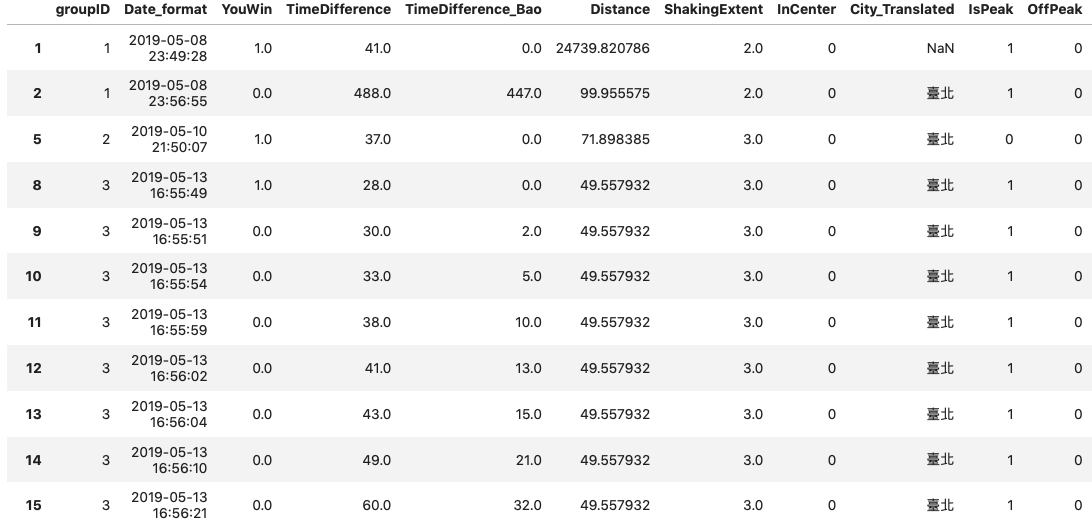
\includegraphics[width=1\textwidth]{Images/data.png}
\end{frame}


%%
\begin{frame}[fragile]{Table of Variables}

\begin{table}[htbp]
\tiny
\begin{tabular}{llll}
Variable            & Description                                      & Type       & 單位     \\
YouWin              & 是否是地震爆文                                          & binary     &        \\
TimeDifference      & 文章發表時間與地震發生時間的時間差                                & continuous & Second \\
TimeDifference\_Bao & 地震文與地震爆文                                         & continuous & second \\
Distance            & 發文者與震央的距離                                        & continuous & km     \\
ShakingExtent       & 震央所在地的震度                                         & level      &        \\
InCenter            & 發文者是否為在震央所在的縣市                                   & binary     &        \\
IsPeak              & 發文者是否在尖峰時段(22:00$\sim$2:00;13:00$\sim$17:00)發文 & binary     &        \\
OffPeak             & 發文者是否在離峰時段(4:00$\sim$8:00; 18:00$\sim$20:00)發文 & binary     &        \\
PopDensity          & 各縣市人口密度                                          & continuous & 人/平方公里 \\
download\_4G        & 各縣市4G移動網路平均下行速率                                  & continuous & Mbps   \\
upload\_4G          & 各縣市4G移動網路平均上行速率                                  & continuous & Mbps  
\end{tabular}

\end{table}
\end{frame}


%%
\begin{frame}[fragile]{About Cleaning Data}

由於由IP位址反查的經緯度僅能定位到「縣市」層級的地理位置,因此與縣市別有關的資料,如:人口密度、4G移動網路下行、上行速率等資料都是以縣市別為單位。

注意到,我們考量的是一場地震的震度,而非規模。因為我們相信震度更能體現體感,即震度能考量到同樣規模下,深、淺層地震給人感受的差別。
又,事實上震度應因縣市而有所不同,然而該資料不易抓取,因此僅納入震央所在地的震度。

\end{frame}

%%
\begin{frame}[fragile]{About Cleaning Data}

尖峰時段與離峰時段的定義方式參考了{\color{blue}\href{https://www.ptt.cc/statistics.html}{PTT Statistics}}的統計數據

將波峰的前後兩小時定義為尖峰時段;將波谷的前後兩小時定義為離峰時段。

	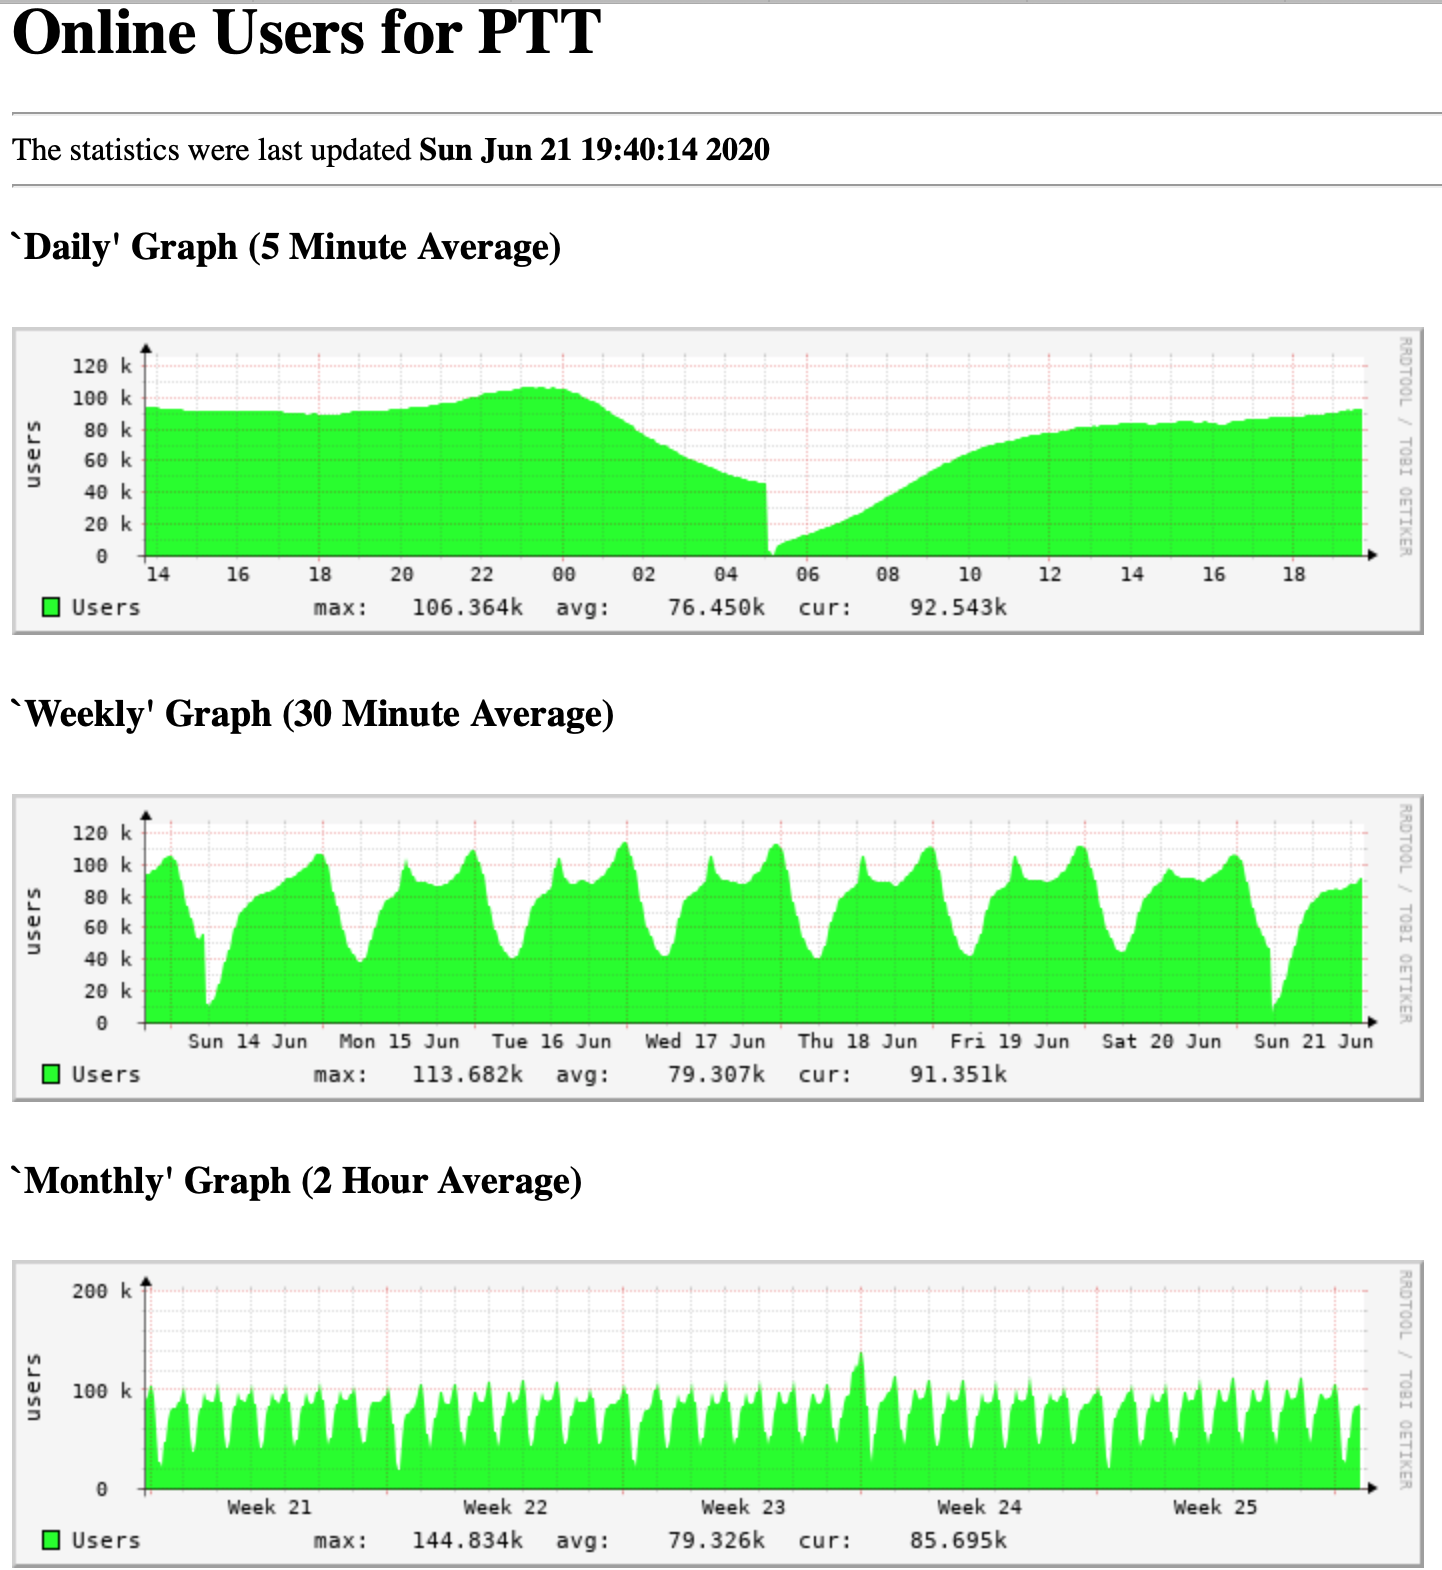
\includegraphics[width=0.5\textwidth]{Images/peak.png}

\end{frame}


%%
\begin{frame}[fragile]{About Cleaning Data}

各縣市的4G移動網路速度來自{\color{blue}\href{https://www.inside.com.tw/article/19538-NCC-4G-speed-report-2019}{NCC發佈的報告}}。

	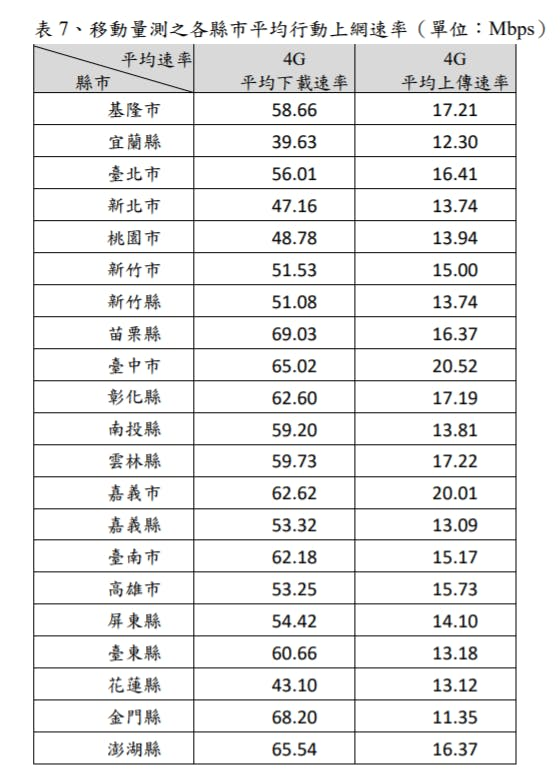
\includegraphics[width=0.5\textwidth]{Images/4g.jpg}

\end{frame}


%%
\begin{frame}[fragile]{About Cleaning Data}

各縣市人口密度資料來自{\color{blue}\href{https://zh.wikipedia.org/wiki/臺灣行政區人口密度表}{Wikipedia}},
由臺灣行政區面積表及臺灣行政區人口列表的資料計算出。

與震央間的距離由經緯度之差{\color{blue}\href{https://wywu.pixnet.net/blog/post/22338038}{簡單換算}}而得:

	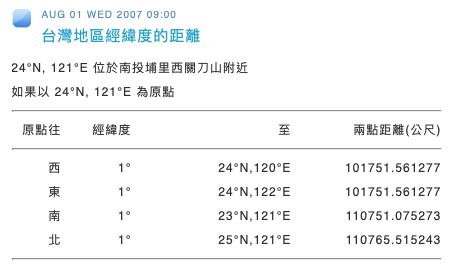
\includegraphics[width=0.7\textwidth]{Images/distance.png}

\end{frame}

